\documentclass[12pt,a4paper]{article}

% ============================================================
% PACKAGES
% ============================================================
\usepackage[
    a4paper,
    top=1.55cm,
    bottom=1.35cm,
    left=1.75cm,
    right=1.75cm
]{geometry}

\usepackage[T1]{fontenc}
\usepackage{newtxtext}
\usepackage{graphicx}
\usepackage{xcolor}
\usepackage{array}
\usepackage{tabularx}
\usepackage{fancyhdr}
\usepackage{tikz}
\usepackage{eso-pic}
\usepackage{ragged2e}

% ============================================================
% COLORS
% ============================================================
\definecolor{GEUBlue}{RGB}{43,91,145}
\definecolor{GEUBannerBlue}{RGB}{0,102,148}
\definecolor{GEUYellow}{RGB}{255,201,38}
\definecolor{InstructionGrey}{RGB}{125,125,125}

% ============================================================
% GENERAL SETTINGS
% ============================================================
\setlength{\parindent}{0pt}
\setlength{\parskip}{0pt}
\renewcommand{\arraystretch}{1}

% ============================================================
% HEADER / FOOTER
% ============================================================
\pagestyle{fancy}
\fancyhf{}

\fancyhead[L]{%
    \fontsize{10.5}{12}\selectfont
    B-Tech OSDBMS-V-2026-T266
}

\fancyhead[R]{%
    \fontsize{10.5}{12}\selectfont
    PHASE-III PROJECT PROGRESS
}

\fancyfoot[R]{%
    \fontsize{10}{12}\selectfont
    Page \thepage
}

\renewcommand{\headrulewidth}{0pt}
\renewcommand{\footrulewidth}{0pt}

\setlength{\headheight}{20pt}
\setlength{\headsep}{0.65cm}
\setlength{\footskip}{0.65cm}

% ============================================================
% BOTTOM YELLOW LINE
% ============================================================
\AddToShipoutPictureBG{%
\begin{tikzpicture}[remember picture,overlay]
    \fill[GEUYellow]
    (current page.south west)
    rectangle
    ([yshift=0.14cm]current page.south east);
\end{tikzpicture}
}

% ============================================================
% CUSTOM COMMANDS
% ============================================================
\newcommand{\sectiontitle}[1]{%
    {\color{GEUBlue}
    \fontsize{18}{22}\selectfont #1}
}

\newcommand{\instruction}[1]{%
    {\color{InstructionGrey}
    \fontsize{10.5}{13}\selectfont #1}
}

% the height given to \answerbox is the minimum height,
% the box grows if the answer is longer
\newcommand{\answerbox}[2]{%
    \begin{tabularx}{\textwidth}{
        |>{\raggedright\arraybackslash}X|}
        \hline
        \setbox0=\hbox{\parbox[t]{\dimexpr\linewidth-12pt\relax}{
            \vspace{5pt}
            \fontsize{11}{13}\selectfont #2}}%
        \ifdim\dimexpr\ht0+\dp0\relax<#1\relax
            \dp0=\dimexpr#1-\ht0\relax
        \fi
        \box0\\
        \hline
    \end{tabularx}
}

% ============================================================
% DOCUMENT
% ============================================================
\begin{document}

% ============================================================
% PAGE 1
% ============================================================

\vspace*{0.10cm}

\includegraphics[width=8.0cm]{geulogo.png}

\vspace{0.70cm}

\noindent
\colorbox{GEUBannerBlue}{%
\parbox{\dimexpr\textwidth-2\fboxsep\relax}{
    \vspace{0.17cm}
    {\color{GEUYellow}
    \fontsize{16.5}{20}\selectfont
    \bfseries
    PROJECT AND TEAM INFORMATION}
    \vspace{0.17cm}
}}

\vspace{0.80cm}

% PROJECT TITLE
\sectiontitle{Project Title}

\vspace{0.05cm}

\vspace{0.40cm}

\answerbox{1.00cm}{High-Throughput Distributed Flash-Sale Transaction Engine}

\vspace{0.80cm}

% TEAM INFORMATION
% \sectiontitle{Student/Team Information}

% \vspace{0.40cm}

% \begin{tabularx}{\textwidth}{
% |>{\raggedright\arraybackslash}p{0.66\textwidth}
% |>{\raggedright\arraybackslash}X|
% }
% \hline

% \parbox[t][1.15cm][t]{\linewidth}{
% \vspace{4pt}
% \fontsize{10.5}{13}\selectfont
% Team Name:\\[2pt]
% Team \# (Mentor needs to assign)
% }
% &
% \\
% \hline

% \parbox[t][3.65cm][t]{\linewidth}{
% \vspace{5pt}
% \fontsize{10.5}{13}\selectfont
% Team member 1 (Team Lead)\\[3pt]
% {\color{InstructionGrey}
% (Last Name, name: student ID: email, picture):}
% }
% &
% \\
% \hline

% \parbox[t][3.65cm][t]{\linewidth}{
% \vspace{5pt}
% \fontsize{10.5}{13}\selectfont
% Team member 2\\[3pt]
% {\color{InstructionGrey}
% (Last Name, name: student ID: email, picture):}
% }
% &
% \\
% \hline

% \end{tabularx}

% \newpage

% ============================================================
% PAGE 2
% ============================================================
\noindent
\begin{tabularx}{\textwidth}{|>{\RaggedRight\arraybackslash}p{0.58\textwidth}|>{\RaggedRight\arraybackslash}X|}
\hline
\begin{minipage}[t]{\linewidth}
\vspace{1.5mm}
\textit{Team Name:}\\[-1mm]
\textit{Team \#}
\vspace{1.5mm}
\end{minipage}
&
\begin{minipage}[t]{\linewidth}
\vspace{1.5mm}
\textit{Hackerblue}
\vspace{1.5mm}
\end{minipage}
\\
\hline
\begin{minipage}[t][3.25cm][t]{\linewidth}
\vspace{1.5mm}
\textbf{Team member 1 (Team Lead)}\\[-1mm]
\vspace{2.0cm}
\end{minipage}
&
\begin{minipage}[t][3.25cm][t]{\linewidth}
\vspace{1.5mm}
\textit{Rana, Priyanshu -- 24021312}\\
\textit{peiyanshurana599@\allowbreak gmail.com}

\vspace{2mm}
\includegraphics[width=3.0cm,height=1.5cm,keepaspectratio]{priyanshu.png}
\end{minipage}
\\
\hline
\begin{minipage}[t][3.25cm][t]{\linewidth}
\vspace{1.5mm}
\textbf{Team member 2}\\[-1mm]
\vspace{2.0cm}
\end{minipage}
&
\begin{minipage}[t][3.25cm][t]{\linewidth}
\vspace{1.5mm}
\textit{Kukreti, Akshit -- 24021085}\\
\textit{KukretiAkshit1869@\allowbreak gmail.com}

\vspace{2mm}
\includegraphics[width=3.0cm,height=1.5cm,keepaspectratio]{Akshit.jpeg}
\end{minipage}
\\
\hline
\begin{minipage}[t][3.25cm][t]{\linewidth}
\vspace{1.5mm}
\textbf{Team member 3}\\[-1mm]
\vspace{2.0cm}
\end{minipage}
&
\begin{minipage}[t][3.25cm][t]{\linewidth}
\vspace{1.5mm}
\textit{Dimri, Sriyam -- 24021413}\\
\textit{sriyamdimri@\allowbreak gmail.com}

\vspace{2mm}
\includegraphics[width=3.0cm,height=1.5cm,keepaspectratio]{sriyam.jpeg}
\end{minipage}
\\
\hline
\end{tabularx}

\newpage
\vspace*{0.15cm}

\noindent
\colorbox{GEUBannerBlue}{%
\parbox{\dimexpr\textwidth-2\fboxsep\relax}{
    \vspace{0.18cm}
    {\color{GEUYellow}
    \fontsize{17}{21}\selectfont
    \bfseries
    PHASE-III PROJECT PROGRESS DESCRIPTION (35 pts)}
    \vspace{0.18cm}
}}

\vspace{0.70cm}

% ABSTRACT
\sectiontitle{Project Abstract}

\vspace{0.05cm}

\vspace{0.12cm}

\answerbox{3.60cm}{
During a flash sale, a lot of customers will want to buy the same few products. This causes issues with the server creating a new thread for each request causing extra CPU overhead. Furthermore, multiple requests will cause the stock to become incorrect, or cause a deadlock.

\vspace{4pt}
The project is a flash sale booking engine which solves this issue. The requests are placed in a bounded queue. Then a limited number of threads are used to handle each request individually. Before the stock is updated, an entry is written to the Write Ahead Log (WAL). Each product has a lock ensuring the stock never goes below 0 and a user cannot buy the same product twice.

\vspace{4pt}
We implemented a Wait For Graph to detect any deadlocks. An admin can start a flash sale via the website and observe the deadlock occurring on the admin page. Locking follows strict two-phase locking, products are found with a B+ Tree and the data can be rebuilt after a crash from the log. The customer store and admin console are both in the browser.
}

\vspace{0.70cm}

% UPDATED APPROACH
\sectiontitle{Updated Project Approach and Architecture}

\vspace{0.05cm}

\vspace{0.25cm}

\answerbox{4.75cm}{
Our proposal said we would write the engine in C++. While building it we moved to Java, so that the engine, the web server and the admin screens could all be made and shown together in one project. The design is the same as in Phase 1: a worker pool, locks, a write-ahead log and a wait-for graph.

\vspace{4pt}
The browser talks to the Java backend with REST calls over HTTP and the data is sent as JSON. Only the standard Java libraries are used (plus the MySQL connector for the optional MySQL mode). The frontend is plain HTML, JavaScript and Tailwind CSS.

\vspace{6pt}
\begin{center}
\resizebox{\linewidth}{!}{%
\begin{tikzpicture}[>=latex,
    blk/.style={draw=GEUBlue, fill=GEUBlue!8, rounded corners=2pt, align=center,
                font=\scriptsize, inner sep=3pt, text width=2.5cm, minimum height=1.3cm},
    wal/.style={blk, draw=GEUYellow!60!black, fill=GEUYellow!25, text width=3.0cm},
    wfg/.style={blk, draw=red!60!black, fill=red!6, text width=3.0cm},
    stp/.style={circle, fill=GEUBannerBlue, text=white, inner sep=1.2pt,
                font=\fontsize{6}{7}\selectfont\bfseries},
    lbl/.style={font=\fontsize{6.5}{8}\selectfont, inner sep=1.5pt, fill=white}]

% ---------- main flow ----------
\node[blk] (users)   at (1.4,0)  {\textbf{Users}\\Customer Store and\\Admin Console\\(browser)};
\node[blk] (server)  at (4.8,0)  {\textbf{Java Web Server}\\REST + JSON\\(16 threads)};
\node[blk] (queue)   at (8.2,0)  {\textbf{Bounded Queue}\\2000 places\\(3 semaphores)};
\node[blk] (workers) at (11.6,0) {\textbf{Worker Threads}\\fixed number\\(2 $\times$ CPU cores)};
\node[blk] (engine)  at (15.0,0) {\textbf{Transaction Engine}\\Strict 2PL locks (S/X)\\B+ Tree index};

\draw[->, thick] (users.east)   -- (server.west)  node[midway, stp] {1};
\draw[->, thick] (server.east)  -- (queue.west)   node[midway, stp] {2};
\draw[->, thick] (queue.east)   -- (workers.west) node[midway, stp] {3};
\draw[->, thick] (workers.east) -- (engine.west)  node[midway, stp] {4};

% answer goes back to the browser
\draw[->, thick, dashed, GEUBannerBlue] (workers.north) -- ++(0,0.9) -| (users.north);
\node[lbl] at (6.5,1.55) {6  answer from the worker (hold, then pay gives a PNR)};

% ---------- lower row ----------
\node[blk, draw=gray, fill=gray!10, text width=2.1cm, anchor=north] (rejected) at (8.2,-1.7) {Rejected\\(queue is full)};
\node[wal, anchor=north] (walbox) at (11.6,-1.7)
  {\textbf{Write-Ahead Log}\\group commit: 1 fsync\\for many records\\snapshot + crash recovery};
\node[wfg, anchor=north] (wfgbox) at (15.0,-1.7)
  {\textbf{Wait-For Graph}\\DFS finds a cycle,\\youngest is rolled back\\sorted lock order};

\node[blk, text width=6.3cm, anchor=north west, align=left] (traffic) at (0,-1.7)
  {\hyphenpenalty=10000\exhyphenpenalty=10000 \textbf{How high traffic is handled}\\
   (a) fixed worker threads, no new thread for every request\\
   (b) the queue takes the burst, extra requests are rejected\\
   (c) lock on every product row: no overselling, one order per user\\
   (d) log records of many orders share one fsync};

\draw[->, dashed, gray] (queue.south) -- (rejected.north);
\node[lbl] at (8.2,-1.2) {full};
\draw[->, thick] (workers.south) -- (walbox.north) node[midway, stp] {5};
\draw[->, thick] (engine.south) -- (wfgbox.north);
\node[lbl] at (15.0,-1.2) {lock waits};
\end{tikzpicture}}

\vspace{2pt}
{\footnotesize \textbf{Figure 1:} Architecture and workflow of the engine. The numbers follow one purchase: (1) the user clicks Buy, (2) the web server puts the request in the queue (it is rejected at once if the queue is full), (3) a worker takes it, (4) the engine takes the product locks and holds the seat for 5 minutes, (5) the log record is on the disk before the answer is given, (6) the worker sends the answer. After payment the order is confirmed with a PNR, an unpaid hold gives the seat back.\par}
\end{center}

\vspace{2pt}
Concurrency control uses strict two-phase locking with our own Lock Manager. A cart takes its locks in sorted order, so a deadlock cannot form, and every wait is reported to the Wait-For Graph, which finds a cycle with a depth first search and rolls back the youngest transaction. A checkpoint snapshot and a replay of the log rebuild the data after a crash.
}

\newpage


% ============================================================
% PAGE 3
% ============================================================

\vspace*{0.20cm}

% TASKS COMPLETED
\sectiontitle{Tasks Completed}

\vspace{0.05cm}

\vspace{0.20cm}

\begin{tabularx}{\textwidth}{
|>{\raggedright\arraybackslash}X
|>{\raggedright\arraybackslash}X|
}
\hline

\textbf{Task Completed} &
\textbf{Team Member}
\\
\hline

\parbox[t]{\linewidth}{\raggedright\vspace{1pt}\fontsize{10.5}{12.5}\selectfont Created the GitHub repository and kept the main branch updated.\vspace{3pt}}
&
\parbox[t]{\linewidth}{\raggedright\vspace{1pt}\fontsize{10.5}{12.5}\selectfont Priyanshu Rana\vspace{3pt}}
\\
\hline

\parbox[t]{\linewidth}{\raggedright\vspace{1pt}\fontsize{10.5}{12.5}\selectfont Implemented bounded queue. Fixed number of workers. Reject if queue is full.\vspace{3pt}}
&
\parbox[t]{\linewidth}{\raggedright\vspace{1pt}\fontsize{10.5}{12.5}\selectfont Priyanshu Rana\vspace{3pt}}
\\
\hline

\parbox[t]{\linewidth}{\raggedright\vspace{1pt}\fontsize{10.5}{12.5}\selectfont Write-ahead log with group commit (many records, one fsync), checkpoints and the log reader.\vspace{3pt}}
&
\parbox[t]{\linewidth}{\raggedright\vspace{1pt}\fontsize{10.5}{12.5}\selectfont Priyanshu Rana\vspace{3pt}}
\\
\hline

\parbox[t]{\linewidth}{\raggedright\vspace{1pt}\fontsize{10.5}{12.5}\selectfont Implement wait for graph. Cycle detection. Rollback victim. Simulate deadlock (any order and sorted order).\vspace{3pt}}
&
\parbox[t]{\linewidth}{\raggedright\vspace{1pt}\fontsize{10.5}{12.5}\selectfont Priyanshu Rana\vspace{3pt}}
\\
\hline

\parbox[t]{\linewidth}{\raggedright\vspace{1pt}\fontsize{10.5}{12.5}\selectfont Lock Manager: strict 2PL with shared and exclusive locks, victim abort and retry.\vspace{3pt}}
&
\parbox[t]{\linewidth}{\raggedright\vspace{1pt}\fontsize{10.5}{12.5}\selectfont Priyanshu Rana\vspace{3pt}}
\\
\hline

\parbox[t]{\linewidth}{\raggedright\vspace{1pt}\fontsize{10.5}{12.5}\selectfont Database layer: B+ Tree index, row locks, hold, payment, PNR and the cart (all or nothing).\vspace{3pt}}
&
\parbox[t]{\linewidth}{\raggedright\vspace{1pt}\fontsize{10.5}{12.5}\selectfont Akshit Kukreti\vspace{3pt}}
\\
\hline

\parbox[t]{\linewidth}{\raggedright\vspace{1pt}\fontsize{10.5}{12.5}\selectfont Crash recovery (snapshot, REDO, UNDO) and the optional MySQL mode with SELECT FOR UPDATE.\vspace{3pt}}
&
\parbox[t]{\linewidth}{\raggedright\vspace{1pt}\fontsize{10.5}{12.5}\selectfont Akshit Kukreti\vspace{3pt}}
\\
\hline

\parbox[t]{\linewidth}{\raggedright\vspace{1pt}\fontsize{10.5}{12.5}\selectfont Customer store: product cards, cart, payment screen with timer, receipt with PNR.\vspace{3pt}}
&
\parbox[t]{\linewidth}{\raggedright\vspace{1pt}\fontsize{10.5}{12.5}\selectfont Sriyam Dimri\vspace{3pt}}
\\
\hline

\parbox[t]{\linewidth}{\raggedright\vspace{1pt}\fontsize{10.5}{12.5}\selectfont Admin console: product management, orders ledger, Engine Core page (Wait-For Graph, performance, burst test, crash recovery).\vspace{3pt}}
&
\parbox[t]{\linewidth}{\raggedright\vspace{1pt}\fontsize{10.5}{12.5}\selectfont Sriyam Dimri\vspace{3pt}}
\\
\hline

\parbox[t]{\linewidth}{\raggedright\vspace{1pt}\fontsize{10.5}{12.5}\selectfont Concurrency, deadlock and recovery tests.\vspace{3pt}}
&
\parbox[t]{\linewidth}{\raggedright\vspace{1pt}\fontsize{10.5}{12.5}\selectfont Sriyam Dimri\vspace{3pt}}
\\
\hline

\end{tabularx}

\vspace{0.65cm}

% CHALLENGES
\sectiontitle{Challenges/Roadblocks}

\vspace{0.05cm}

\vspace{0.18cm}

\answerbox{4.05cm}{
\textbf{1. Deadlock never happens on its own.} A purchase takes only one product lock, so the Wait-For Graph was always empty. We built a simulation that the admin starts from the website: 2 to 5 buyer threads, each takes a lock and then asks for the lock of the next buyer. A barrier makes the circular wait always form. A second mode takes the locks in sorted order and never deadlocks.

\vspace{2pt}
\textbf{2. Keeping the stock correct.} Many threads can read the same stock value together and oversell. A plain lock was not enough for carts, so we wrote a Lock Manager with strict two-phase locking (shared and exclusive locks).

\vspace{2pt}
\textbf{3. WAL speed.} An fsync after every record is safe but slow. Group commit fixed it: one fsync writes the records of many orders (about 45 records per fsync in our burst test).

\vspace{2pt}
\textbf{4. Crash recovery.} A snapshot is saved at every checkpoint. After a crash the log after it is replayed (REDO) and unpaid holds give their seats back (UNDO).

\vspace{2pt}
\textbf{5. Change from C++ to Java.} The proposal said C++, but the engine is in Java, so some parts changed. For example, the pre-allocated memory buffer is not used.
}

\vspace{0.65cm}

% TASKS PENDING
% \sectiontitle{Tasks Pending (7 pts)}

% \vspace{0.05cm}

% \instruction{
% (Describe the main tasks that you still need to complete.
% Max 250 words).
% }

% \vspace{0.18cm}

% \begin{tabularx}{\textwidth}{
% |>{\raggedright\arraybackslash}X
% |>{\raggedright\arraybackslash}X|
% }
% \hline

% \textbf{Task Pending} &
% \textbf{Team Member (to complete the task)}
% \\
% \hline

% \parbox[t][1.25cm][t]{\linewidth}{}
% &
% \parbox[t][1.25cm][t]{\linewidth}{}
% \\
% \hline

% \end{tabularx}

\newpage

% ============================================================
% PAGE 4
% ============================================================

\vspace*{0.30cm}

% OUTCOMES
\sectiontitle{Project Outcome/Deliverables}

\vspace{0.05cm}

\vspace{0.35cm}

\answerbox{3.35cm}{
The final outcome is a working flash sale engine with a web interface. The main deliverables are:

\vspace{2pt}
$\bullet$ \textbf{Core engine:} worker pool, strict 2PL lock manager, B+ Tree index, write-ahead log with group commit and the Wait-For Graph, written in Java.\\
$\bullet$ \textbf{Customer store and admin console:} seat hold with a 5 minute timer, payment, PNR, cart, product management and a live view of the engine.\\
$\bullet$ \textbf{Concurrency tests:} they show that the final stock is always correct, with no overselling and no duplicate orders.\\
$\bullet$ \textbf{Deadlock testing:} the admin starts the buyer threads and sees the deadlock, its recovery and the prevention by sorted lock order.\\
$\bullet$ \textbf{Performance numbers:} latency, p95, lock wait, records per fsync and a burst test with thousands of users.\\
$\bullet$ \textbf{Crash recovery test:} the data is rebuilt from the snapshot and the WAL file.
}

\vspace{0.75cm}

% PROGRESS
\sectiontitle{Progress Overview}

\vspace{0.05cm}

\vspace{0.25cm}

\answerbox{4.45cm}{
The project is almost complete, about 95 percent. Everything we planned in Phase 1 is built and tested: the queue and workers, strict two-phase locking, the B+ Tree, the WAL with group commit, the Wait-For Graph with recovery and prevention, crash recovery, the seat hold with payment and PNR, and the full web interface.

\vspace{2pt}
\textbf{Ahead of schedule:} the admin deadlock simulation in two modes, the product edit feature, the cart, the burst test and the crash recovery button. These were not in our first plan.

\vspace{2pt}
\textbf{Remaining:} the MySQL mode is written but we have not run it against a live MySQL server yet. We will test it before the final demo. The engine works without MySQL, so nothing else depends on it.
}

\vspace{0.75cm}

% ============================================================
% PAGE 5
% ============================================================

\vspace*{0.20cm}

% CODEBASE
\sectiontitle{Codebase Information}

\vspace{0.05cm}

\vspace{0.20cm}

\answerbox{3.70cm}{
\textbf{Repository:}\\
{\raggedright\texttt{https://github.com/priyanshu24021312/\allowbreak High-Throughput-Distributed-\allowbreak Flash-Sale-Transaction-Engine}\par}

\vspace{2pt}
\textbf{Branch:} main (the only branch, 7 commits so far)

\vspace{2pt}
\textbf{Important commits:}\\
$\bullet$ Initial commit (about 2 months ago): created the repository.\\
$\bullet$ Add flash sale engine code (last month): first version of the engine, with the B+ Tree and Database classes.\\
$\bullet$ feat: add flash sale frontend and project interface (3 weeks ago): customer and admin website.\\
$\bullet$ feat: integrate wait-for graph deadlock detection and recovery, commit \texttt{2e980c7} (5 days ago): the previous commit.

\vspace{2pt}
The Lock Manager, the new B+ Tree, group commit, crash recovery, the seat hold with payment and the burst test come in the next commit.
}

\vspace{0.65cm}

\newpage

% TESTING
\sectiontitle{Testing and Validation Status}

\vspace{0.05cm}

\vspace{0.30cm}

\begin{tabularx}{\textwidth}{
|>{\raggedright\arraybackslash}p{0.27\textwidth}
|>{\raggedright\arraybackslash}p{0.13\textwidth}
|>{\raggedright\arraybackslash}X|
}
\hline

\textbf{Test Type} &
\textbf{Status (Pass/Fail)} &
\textbf{Notes}
\\
\hline

\parbox[t]{\linewidth}{\raggedright\vspace{1pt}\fontsize{10.5}{12.5}\selectfont Concurrency (overselling) test\vspace{3pt}}
&
\parbox[t]{\linewidth}{\raggedright\vspace{1pt}\fontsize{10.5}{12.5}\selectfont Pass\vspace{3pt}}
&
\parbox[t]{\linewidth}{\raggedright\vspace{1pt}\fontsize{10.5}{12.5}\selectfont 60 threads on 15 units: exactly 15 holds. Burst of 6000 users on 30 units: 30 booked, the rest sold out or rejected by the full queue, none lost.\vspace{3pt}}
\\
\hline

\parbox[t]{\linewidth}{\raggedright\vspace{1pt}\fontsize{10.5}{12.5}\selectfont Duplicate purchase test\vspace{3pt}}
&
\parbox[t]{\linewidth}{\raggedright\vspace{1pt}\fontsize{10.5}{12.5}\selectfont Pass\vspace{3pt}}
&
\parbox[t]{\linewidth}{\raggedright\vspace{1pt}\fontsize{10.5}{12.5}\selectfont Same user buying the same product twice: the second request was rejected.\vspace{3pt}}
\\
\hline

\parbox[t]{\linewidth}{\raggedright\vspace{1pt}\fontsize{10.5}{12.5}\selectfont Lock Manager (strict 2PL)\vspace{3pt}}
&
\parbox[t]{\linewidth}{\raggedright\vspace{1pt}\fontsize{10.5}{12.5}\selectfont Pass\vspace{3pt}}
&
\parbox[t]{\linewidth}{\raggedright\vspace{1pt}\fontsize{10.5}{12.5}\selectfont S+S allowed, X blocks S and X, S to X upgrade works. 8 threads x 2000 increments gave exactly 16000.\vspace{3pt}}
\\
\hline

\parbox[t]{\linewidth}{\raggedright\vspace{1pt}\fontsize{10.5}{12.5}\selectfont Deadlock detection (Wait-For Graph)\vspace{3pt}}
&
\parbox[t]{\linewidth}{\raggedright\vspace{1pt}\fontsize{10.5}{12.5}\selectfont Pass\vspace{3pt}}
&
\parbox[t]{\linewidth}{\raggedright\vspace{1pt}\fontsize{10.5}{12.5}\selectfont 2, 3 and 5 buyer threads: the cycle was found every time and shown on the admin page.\vspace{3pt}}
\\
\hline

\parbox[t]{\linewidth}{\raggedright\vspace{1pt}\fontsize{10.5}{12.5}\selectfont Deadlock recovery\vspace{3pt}}
&
\parbox[t]{\linewidth}{\raggedright\vspace{1pt}\fontsize{10.5}{12.5}\selectfont Pass\vspace{3pt}}
&
\parbox[t]{\linewidth}{\raggedright\vspace{1pt}\fontsize{10.5}{12.5}\selectfont Youngest buyer rolled back (DEADLOCK\_VICTIM), the others booked, then the victim retried and booked too. Resolves by itself after 30 seconds.\vspace{3pt}}
\\
\hline

\parbox[t]{\linewidth}{\raggedright\vspace{1pt}\fontsize{10.5}{12.5}\selectfont Deadlock prevention (sorted lock order)\vspace{3pt}}
&
\parbox[t]{\linewidth}{\raggedright\vspace{1pt}\fontsize{10.5}{12.5}\selectfont Pass\vspace{3pt}}
&
\parbox[t]{\linewidth}{\raggedright\vspace{1pt}\fontsize{10.5}{12.5}\selectfont Carts [2,3] and [3,2] asked 3000 times: no deadlock. The simulation in sorted mode never deadlocks.\vspace{3pt}}
\\
\hline

\parbox[t]{\linewidth}{\raggedright\vspace{1pt}\fontsize{10.5}{12.5}\selectfont B+ Tree index\vspace{3pt}}
&
\parbox[t]{\linewidth}{\raggedright\vspace{1pt}\fontsize{10.5}{12.5}\selectfont Pass\vspace{3pt}}
&
\parbox[t]{\linewidth}{\raggedright\vspace{1pt}\fontsize{10.5}{12.5}\selectfont 20000 random insert, delete and search operations matched a TreeMap. 4 writers and 4 readers together: nothing lost.\vspace{3pt}}
\\
\hline

\parbox[t]{\linewidth}{\raggedright\vspace{1pt}\fontsize{10.5}{12.5}\selectfont WAL and group commit\vspace{3pt}}
&
\parbox[t]{\linewidth}{\raggedright\vspace{1pt}\fontsize{10.5}{12.5}\selectfont Pass\vspace{3pt}}
&
\parbox[t]{\linewidth}{\raggedright\vspace{1pt}\fontsize{10.5}{12.5}\selectfont TXN\_BEGIN, ORDER\_COMMIT and TXN\_ABORT are in data/wal.log. 400 concurrent commits needed far fewer fsyncs (177).\vspace{3pt}}
\\
\hline

\parbox[t]{\linewidth}{\raggedright\vspace{1pt}\fontsize{10.5}{12.5}\selectfont Hold, payment and expiry\vspace{3pt}}
&
\parbox[t]{\linewidth}{\raggedright\vspace{1pt}\fontsize{10.5}{12.5}\selectfont Pass\vspace{3pt}}
&
\parbox[t]{\linewidth}{\raggedright\vspace{1pt}\fontsize{10.5}{12.5}\selectfont Pay gives a PNR. Cancel and the 5 minute timeout give the seat back. Paying twice or after expiry is refused.\vspace{3pt}}
\\
\hline

\parbox[t]{\linewidth}{\raggedright\vspace{1pt}\fontsize{10.5}{12.5}\selectfont Cart (all or nothing)\vspace{3pt}}
&
\parbox[t]{\linewidth}{\raggedright\vspace{1pt}\fontsize{10.5}{12.5}\selectfont Pass\vspace{3pt}}
&
\parbox[t]{\linewidth}{\raggedright\vspace{1pt}\fontsize{10.5}{12.5}\selectfont One sold-out item fails the whole cart and nothing is reserved.\vspace{3pt}}
\\
\hline

\parbox[t]{\linewidth}{\raggedright\vspace{1pt}\fontsize{10.5}{12.5}\selectfont Crash recovery\vspace{3pt}}
&
\parbox[t]{\linewidth}{\raggedright\vspace{1pt}\fontsize{10.5}{12.5}\selectfont Pass\vspace{3pt}}
&
\parbox[t]{\linewidth}{\raggedright\vspace{1pt}\fontsize{10.5}{12.5}\selectfont Server killed with kill -9 and started again: products, 10 confirmed orders and PNRs identical, unpaid holds undone. The Simulate Crash button shows the same state before and after.\vspace{3pt}}
\\
\hline

\parbox[t]{\linewidth}{\raggedright\vspace{1pt}\fontsize{10.5}{12.5}\selectfont Admin edit product test\vspace{3pt}}
&
\parbox[t]{\linewidth}{\raggedright\vspace{1pt}\fontsize{10.5}{12.5}\selectfont Pass\vspace{3pt}}
&
\parbox[t]{\linewidth}{\raggedright\vspace{1pt}\fontsize{10.5}{12.5}\selectfont Name, price, description and quantity change, sold tickets stay counted. Empty name or price 0 is rejected.\vspace{3pt}}
\\
\hline

\parbox[t]{\linewidth}{\raggedright\vspace{1pt}\fontsize{10.5}{12.5}\selectfont Browser test of the website\vspace{3pt}}
&
\parbox[t]{\linewidth}{\raggedright\vspace{1pt}\fontsize{10.5}{12.5}\selectfont Pass\vspace{3pt}}
&
\parbox[t]{\linewidth}{\raggedright\vspace{1pt}\fontsize{10.5}{12.5}\selectfont Hold, pay, cancel, cart, expiry, ledger, burst test, crash recovery and both deadlock modes. No errors in the browser.\vspace{3pt}}
\\
\hline

\parbox[t]{\linewidth}{\raggedright\vspace{1pt}\fontsize{10.5}{12.5}\selectfont MySQL mode\vspace{3pt}}
&
\parbox[t]{\linewidth}{\raggedright\vspace{1pt}\fontsize{10.5}{12.5}\selectfont Pending\vspace{3pt}}
&
\parbox[t]{\linewidth}{\raggedright\vspace{1pt}\fontsize{10.5}{12.5}\selectfont Written (ACID transaction with SELECT FOR UPDATE) but not tried with a live MySQL server yet. All tests above used the in-memory mode.\vspace{3pt}}
\\
\hline

\end{tabularx}

\newpage

% DELIVERABLES
\sectiontitle{Deliverables Progress}

\vspace{0.05cm}

\vspace{0.25cm}

\answerbox{3.20cm}{
$\bullet$ \textbf{Core engine} (worker pool, 2PL locks, B+ Tree, WAL, Wait-For Graph): \textbf{Completed}\\
$\bullet$ \textbf{Customer store and admin console} (hold, payment, PNR, cart): \textbf{Completed}\\
$\bullet$ \textbf{Concurrency tests:} \textbf{Completed}\\
$\bullet$ \textbf{Deadlock testing} (detection, recovery, prevention): \textbf{Completed}\\
$\bullet$ \textbf{Performance numbers} (latency, lock wait, group commit, burst test): \textbf{Completed}\\
$\bullet$ \textbf{Crash recovery test} (kill -9 and Simulate Crash button): \textbf{Completed}\\
$\bullet$ \textbf{MySQL mode with a live server:} \textbf{Pending.} Code is written, the test is still to do.
}

\end{document}
